% (c) Jakub Stejskal
% Master Thesis
% Performance Testing and Analysis of Qpid-Dispatch Router
% Chapter 5
\chapter{Implementation}
\label{Implementation}
This chapter summarizes the implementation of components, which were described in the Chapter \ref{Analysis and Design}. The main part is the Agent module for MPT, which is implemented in Java and Groovy language. The second part is Topology Generator, which is python package for automatic generation of dispatch topology based on user's metadata. Since topology deployment is not part MPT or Topology Generator, there is also described \emph{Ansible} and \emph{Docker} technology. Measurement data gathering and reporting is done by MPT parts which already been mentioned in the Chapter \ref{Analysis and Design}.


\section{Used Technologies}
Messaging Performance Tool is a very large project with several parts. The most of MPT, such as command parsing, reporting, clients abstractions and so on, are written in Java language. But it is not pure Java code. For specify the test, which using MPT, is used Groovy language. Groovy is basically lightweight version of Java with several advantages. From my point of view are Groovy scripts more readable for those who are not more familiar with Java code. Groovy scrips are also used as reaction for specific commands for extension points, but this is deeply described in the Subsection \ref{MPT Preparations}.

On the other hand, Topology Generator is a new simple project. For easy integration to another projects, quick development and easy code preview I choose \emph{Python} language. Whole generator is created as one package, which is available for install on every machine with installed Python version 2.7 and higher. Already mentioned technologies are very common and almost every programmer have heard about Java and Python. In the following subsections I describe technologies, which are not common, but they are widely in use.

\subsection{Ansible}
Ansible \cite{Ansible} is simple automation framework which allow users to automate daily tasks on multiple nodes or containers. Basic types of tasks which can be automated by Ansible are:

\begin{itemize}
	\item \textbf{Provisioning}\,---\,setup the various servers user need in network infrastructure.
	\item \textbf{Configuration management}\,---\,change configuration of an application, operation system or device. Basically it allows start, stop and restart services, install or update application or perform a wide variety of other configuration tasks.
	\item \textbf{Application deployment}\,---\,automatic deployment of internally developed application to your systems with all dependencies.
\end{itemize}

Ansible scripts are written in YAML language which makes Ansible scripts to easy readable for humans and very simple to manage. Another advantage is that user does not even need to know commands used to accomplish a particular tasks. All is needed to specify what state does user wants the system to be in. Ansible is available on multiple systems with really short list of dependencies; Linux based systems needs Python and Windows need PowerShell, both systems needs SSH.

\begin{figure}[H]
  \centering
  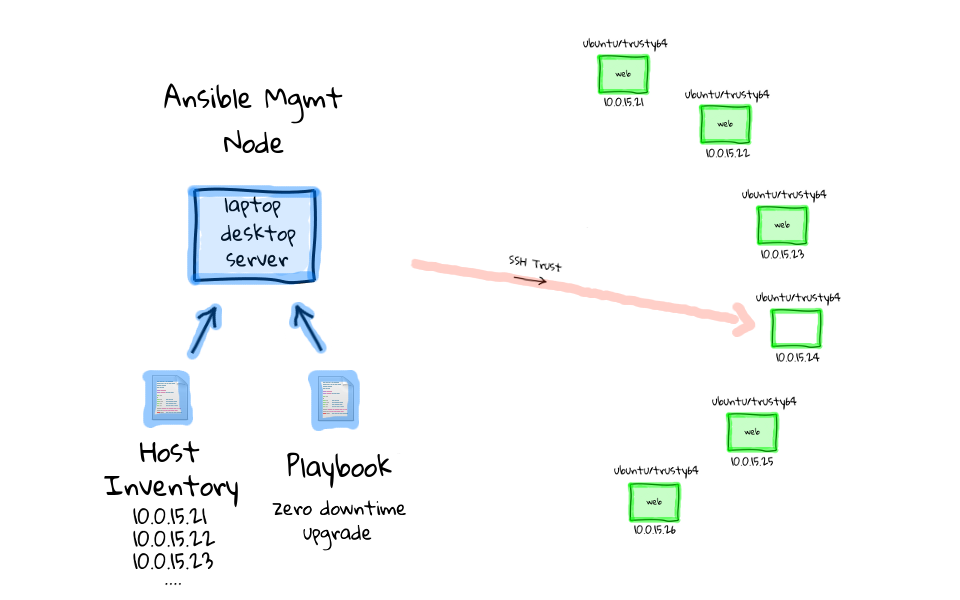
\includegraphics[width=10cm]{obrazky-figures/ansible.png}
  \caption{Ansible architecture. \todo{Placeholder}}
  \label{fig:ansible_architecture}
\end{figure}

In this thesis is Ansible used for several tasks; main is to deploy systems on specific nodes. As I want to run performance tests of Qpid-dispatch on multiple topology scenarios it is necessary to do system deployment quickly and automated which is easy with Ansible. System deployment contains MPT installation, Qpid-dispatch installation and other services based on testing scenario. The next task is to create and deploy configuration files for each router machine. This task runs Topology generator and based on its output create configuration file for each machine.


\subsection{Docker}
Docker \cite{Docker} is an open platform which provide developing, shipping and running application separately from your infrastructure. Basically, docker is specific type of virtualization technology which allows the ability to package and run an application in a loosely isolated environment called a container. Docker containers are lightweight virtual machines run directly within the host machine's kernel. This means that you can run more containers than virtual machines on specific hardware, even you can run containers on virtual machines.

Docker container are build up from a dockerfile where are specified container attributes such as OS in container, environment variables and steps for install applications. Output of build command is docker image. This image is ready for run as a container with another specific attributes such as exposes ports. Containers can be attach to same network which allow communication between all containers in the same network.

\begin{figure}[H]
  \centering
  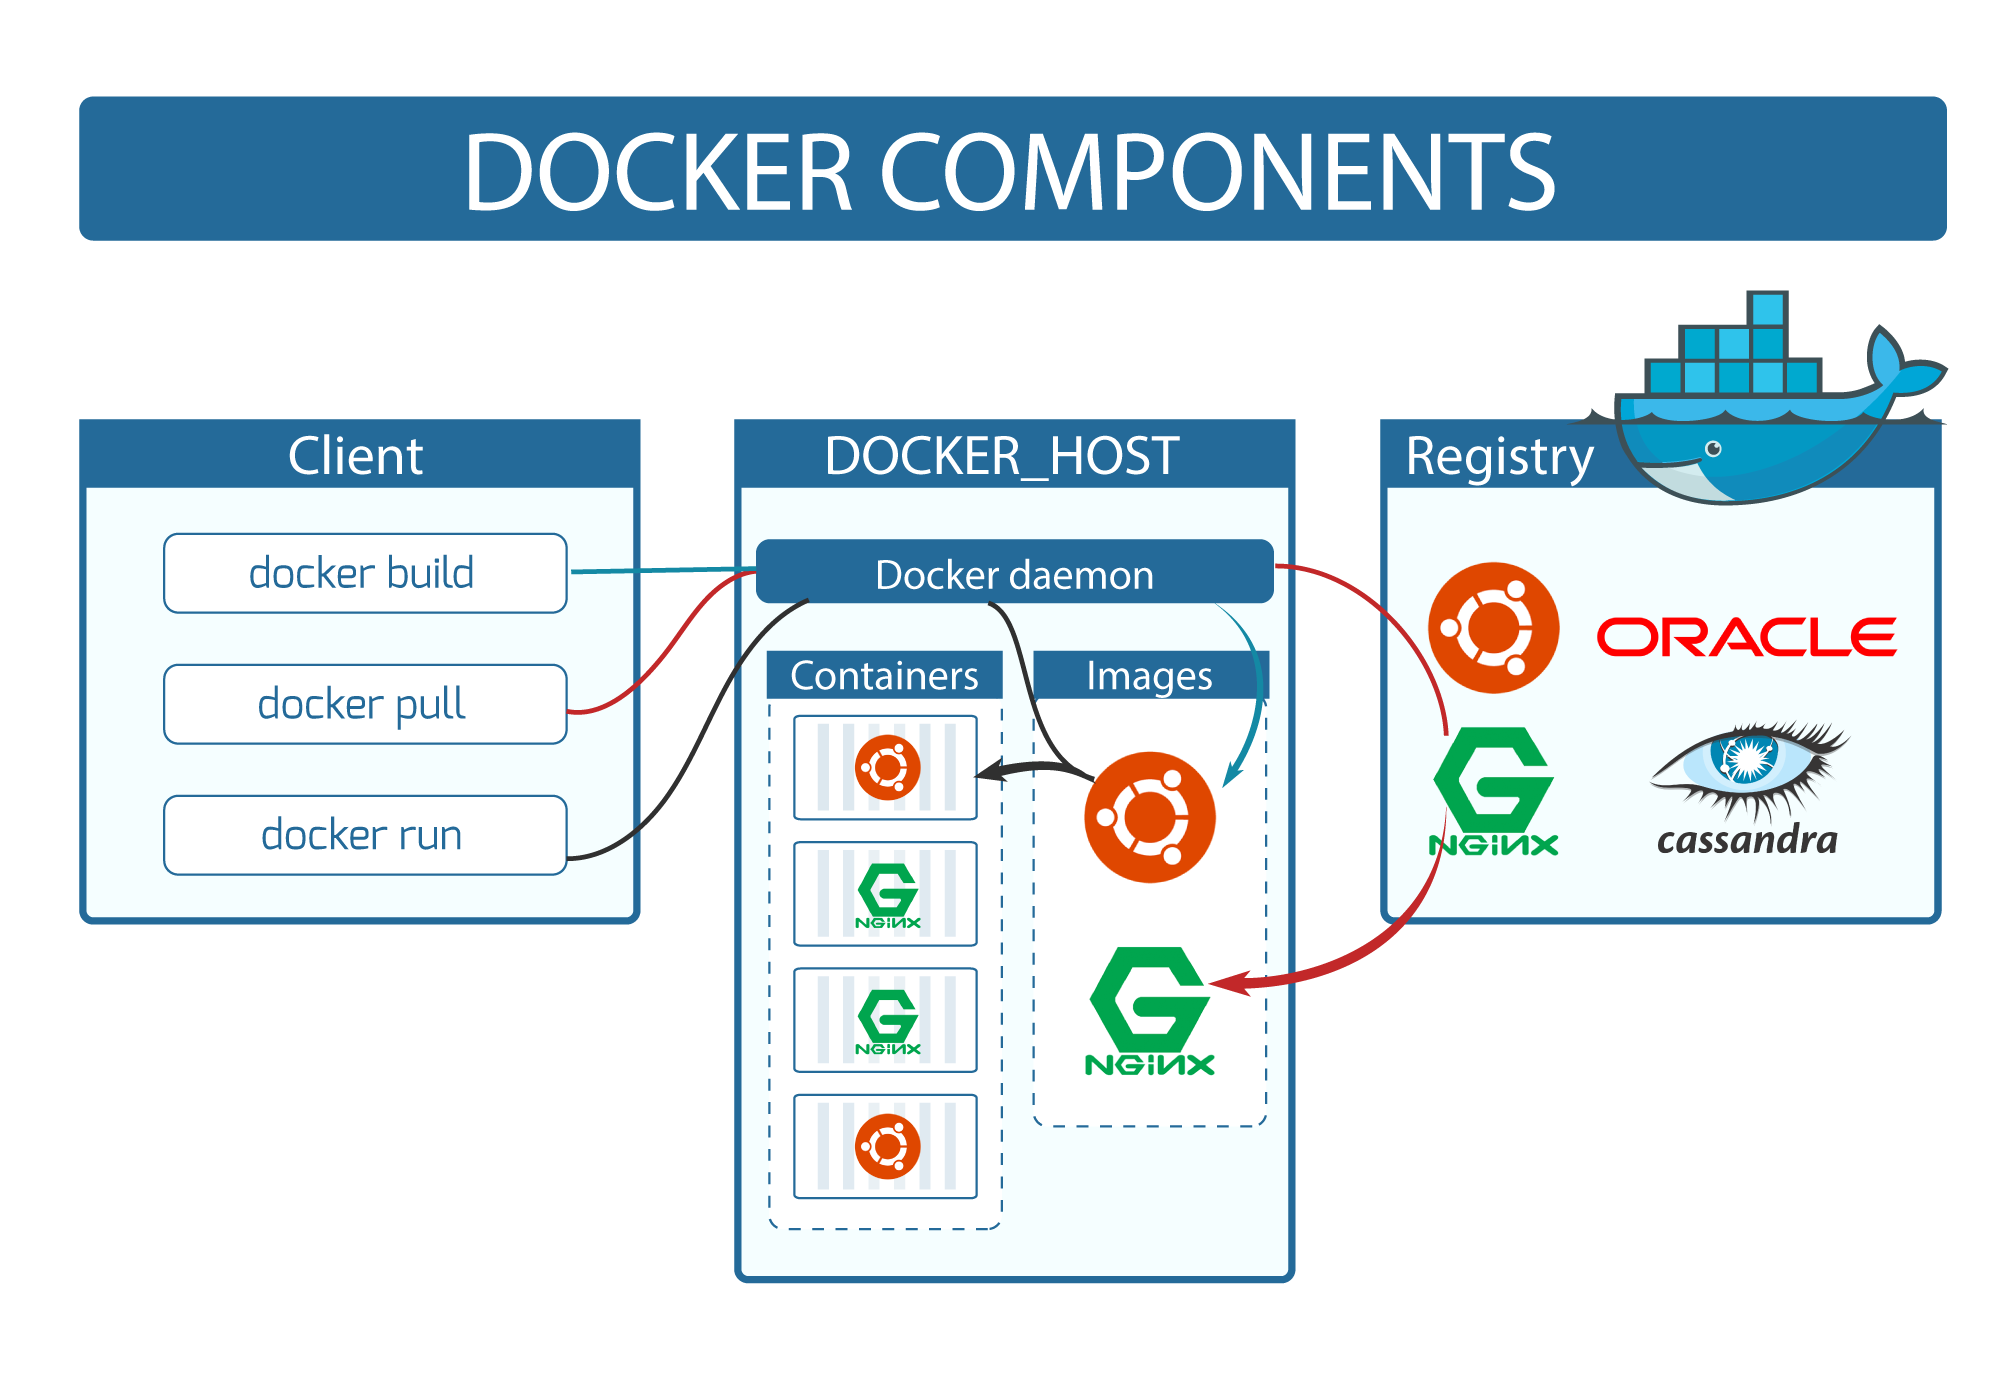
\includegraphics[width=10cm]{obrazky-figures/docker.png}
  \caption{Docker architecture. \todo{Placeholder}}
  \label{fig:ansible_architecture}
\end{figure}


Since docker is able to run services such as Qpid-dispatch very easily and also allow communication between containers, we are able to deploy MPT with proper SUT on containers and analyze behavior in the container network or just run MPT on single machine. However, for proper performance results we needs real machines, docker containers are uses only for testing and trying some basic stuffs with MPT.


\section{Topology Generation}
Qpid-dispatch has a lot of configurable attributes, which can influence router behavior. These attributes can be setup with an AMQP management tool called \emph{qdmanage}\footnotemark or you can specify them directly in the configuration file. Since qdmanage needs human interaction, it is more comfortable to create configuration file for each specific test case. Here comes Topology Generator on the scene.

\footnotetext{qdmanage - \url{https://qpid.apache.org/releases/qpid-dispatch-1.0.1/man/qdmanage.html}}

In case of network with multiple router, it is uncomfortable to update configuration file for each router and then do a deployment. An idea of Topology Generator introduce an option to update only single file with router specification and leave generation and deployment on automated approach. However, the generation and deployment takes few simple steps to achive proper teoplogy changes. These steps are described in the following Subsections.

\subsection{Configuration File Generation}
At first, you should realize that each configuration file is not generated by Topology Generator itself by it is generated by Ansible playbook. Why this approach? Since Qpid-dispatch is getting new versions every few months, new version can change names of any configuration attribute or even can erase them. This cause the problem, that when is Qpid-dispatch updated, the code of Topology Generator has to be reviewed and updated too or you risk syntax error in configuration file. This approach is not very stable. Simple solution is let Ansible to do final generation.

The trick is, that Ansible is able to fill-up any kind of passed \emph{Jinja2}\footnotemark template only with data which are available. Basically, Ansible script will get configuration template and variables for router configuration files. Now, script simply iterate through template and fill-up all available attributes. You can see the pseudocode of this process in the Algortihm \ref{alg:ansible_template_fill}.

\begin{center}
	\begin{algorithm}[H]
		 % \KwData{this text}
		 \KwResult{Filled template - configuration file}
		 load variables for configuration files\;
		 load configuration file template\;
		 \While{not at end of template}{
			  read line with specific variable to fill\;
			  \eIf{know current variable}{
				   fillup the variable\;
			   }{
					 erase current line\;
				 }
				go to the next line\;
		 }
		 \caption{Config template fill-up by Ansible script.}
		 \label{alg:ansible_template_fill}
	\end{algorithm}
\end{center}

This process is done for every router machine in your inventory file. Since configuration variables are in JSON format, Ansible can recognize which variables are for each machine.

\footnotetext{Jinja2 - \url{http://jinja.pocoo.org/docs/2.10/}}

\subsection{Template Generator}
Configuration file are strictly based on configuration template. That means, that Ansible needs template with specific atributes for each version. However, Qpid-dispatch offers smart solution how to get this template. Attributes are available inside a JSON file in the installation folder of Qpid-dispatch. For process this JSON file and create configuration template we used simple tool called \emph{qdrouter-jinja2}\footnotemark.

Qpid-dispatch configuration file is divided into multiple section where each section has its own attributes. For example there is a \emph{router} section with router name, mode, etc., and \emph{ssl} section with security attributes. Each section can be specified multiple times, but usually is only the last one used. The exceptions are \emph{connectors}, \emph{listeners}, \emph{addresses} and \emph{link routes} which can specify multiple connection points and routing types on single router. In the Algorithm \ref{alg:ansible_template_generator} you can see pseudocode of template generation process.

\begin{center}
	\begin{algorithm}[H]
		 \KwData{Attributes in JSON}
		 \KwResult{Configuration template}
		 load JSON file\;
		 create Jinja2 output file\;
		 \While{not at end of JSON}{
			  read line\;
			  \uIf{it is section name}{
				   wrap line with section Jinja2 code\;
					 put wrapped line into output\;
			  }
			 	\uElseIf{it is attribute name}{
					 wrap line with attribute Jinja2 code\;
					 put wrapped line into output\;
			 	}
				\Else{
					put line into output\;
				}
		 }
		 remove multiple blank lines\;
		 \caption{Template generation by qdrouter-jinja2.}
		 \label{alg:ansible_template_generator}
	\end{algorithm}
\end{center}

From pseudocode you can see that there are two kind of wrappers for parsing JSON. Their function is to make config sections and attributes optional and repeatable which is achieve by wrap the sections and attributes with Jinja2 code. The attribute wrapper process each attribute line into the following:

\begin{verbatim}
{%% if section.attribute is defined %%}
    attribute: {{ section.attribute }}
{%% endif %%}
\end{verbatim}

This code in template means, that if Ansible knows the variable \emph{section.attribute}, it add a line with that attribute name and variable value into config file. Key words section and attribute are just placeholders for real name such as \emph{connector} for section and \emph{host} for attribute. Output can looks like the following line:

\begin{verbatim}
		host: 10.0.0.1
\end{verbatim}

The section wrapper is more complex, because it is needed to wrap start of the section and end of the section. This is handled by class methods \textbf{\textunderscore enter\textunderscore ()} and \textbf{\textunderscore exit\textunderscore ()} which allows you to implement objects that execute \textbf{\textunderscore enter\textunderscore ()} at start and \textbf{\textunderscore exit\textunderscore ()} at the end of some statement. Basically is that class created for each section and methods are invoked before first and after last attribute. Method \textbf{\textunderscore enter\textunderscore ()} wrap start of each section with following code:

\begin{verbatim}
{%% if item.section_name is defined %%}
{%% for section_name in item.section_name %%}
section_name {
\end{verbatim}

The \textbf{\textunderscore exit\textunderscore ()} method wrapper add following piece of code into Jinja2 template:
\begin{verbatim}
}


\end{verbatim}

Since qdrouter-jinja2 parse JSON data from installed version of Qpid-dispatch on remote node it can guarantee that template will always corespond with specific router version. The template is saved in \emph{/tmp} folder on remote machine where Ansible scripts can fetch it into local folder and fill-up with data.

\footnotetext{qdrouter-jinja2 - \url{https://github.com/rh-messaging-qe/qdrouter-jinja2}}

\subsection{Topology Generator}
Topology Generator is the main part of configuration generation and deployment. It takes care about configuration variables for Ansible deployment scripts from user specification. Topology Generator needs two parameters, path to inventory, and path to graph file or topology type:

\begin{description}
	\item \textbf{Path to Inventory}\,---\,Inventory is simple config file with list of nodes, connected to your network. Generator gets nodes name and type (router, broker) and use them during variables generation. The generator create specific sections and attributes based on node type and graph type. Since broker configs are not generated by this tool, it use information about only for specification of link routes to neighbours.
	\item \textbf{Path to Graph file}\,---\,Graph file is simple YAML file which specify node distribution in the network. It contain at least node name and links to another nodes. Beside the name, user can specify another node informations such as constructors, listeners, ssl profiles, etc. very easily for each node. Whole file is load during initialization and it is processed with generator.
	\item \textbf{Topology Type}\,---\,Generator can create topology without graph file, but needs network type which will generate. For example network type can be a line which puts all nodes into one line and generate connections between them.
\end{description}

Inner representation of network is done via python library \emph{NetworkX}\footnotemark. It creates a graph as an object and offers manipulation with its attributes which are objects of nodes and links. Generator is able to store information about network configuration as an attributes of these objects. During graph initialization, the generator store basic information about nodes such as name and type from inventory or some additional information from graph file. Basic algortihm of topology generation is available on the Algorithm \ref{alg:ansible_tology_generator_1}.

\begin{center}
	\begin{algorithm}[H]
		 \KwData{Inventory, Graph File/Topology Type}
		 \KwResult{Configuration variables in JSON}
		 load and parse Inventory\;
		 create inner representation of topology based on input parameters\;
		 \ForEach{node}{
		 		\ForEach{config section}{
				  \If{generate default attributes}{
					   generate default attributes based on connections inside network\;
						 add generated facts into dictionary\;
				  }
					generate attributes based on data from graph file\;
					add generated facts into dictionary\;
				}
		 }
		 print facts dictionary into file\;
		 \caption{Basic steps during topology generation.}
		 \label{alg:ansible_tology_generator_1}
	\end{algorithm}
\end{center}

\footnotetext{NetworkX - \url{https://networkx.github.io/documentation/latest/}}

However, the generation for each config section is more complex and it is slightly different for sections that cares about connection to another nodes.
\TODO{dopsat}

\subsection{Deployment}
Ansible play

\section{Qpid-Dispatch Performance Module}

\subsection{MPT Preparations}
\label{MPT Preparations}

\subsection{Agent Module Integration}

\subsection{Groovy As an Extension Handler}

\subsection{Agent Capabilities}
